\documentclass[15pt,a4paper]{article}

%use the english line for english reports
%usepackage[english]{babel}
\usepackage[portuguese]{babel}
\usepackage[utf8]{inputenc}
\usepackage{indentfirst}
\usepackage{graphicx}
\usepackage{moreverb}
\usepackage{subfig}
\usepackage{float}
\usepackage{url}

\floatstyle{ruled}
\newfloat{code}{!ht}{lop}
\floatname{code}{Código fonte}


\begin{document}

\setlength{\textwidth}{16cm}
\setlength{\textheight}{22cm}


%************************************************************************************************
%************************************************************************************************

\title{
	\Huge\textbf{Breakthrough}
	\linebreak\linebreak\linebreak
	\Large\textbf{Relatório Intercalar}
	\linebreak\linebreak
	
\includegraphics[height=6cm, width=7cm]{feup.pdf}
	\linebreak \linebreak
	\Large{Mestrado Integrado em Engenharia Informática e Computação}
	\linebreak\linebreak
	\Large{Programação em Lógica}\linebreak
}


\author{\textbf{Grupo 17:}
\\ João Guedes - 070509043
\\ João Henriques - 110509026
\\\linebreak\linebreak \\
\\ Faculdade de Engenharia da Universidade do Porto
\\ Rua Roberto Frias, s\/n, 4200-465 Porto, Portugal
\linebreak\linebreak\linebreak
\linebreak\linebreak\vspace{1cm}}
\date{Setembro de 2011}
\maketitle
\thispagestyle{empty}



%************************************************************************************************
%************************************************************************************************


\section*{Resumo}

% Descrever muito sumariamente o trabalho. Deve ser suficiente para o leitor decidir se lê ou não o resto do relatório.
% Não deve incluir nenhuma referência ao facto de ser feito no âmbito de uma cadeira.



O \textit{Breakthrough} é um jogo de tabuleiro tradicional semelhante às damas, premiado e com um conjunto de regras muito simples e acessível.

A implementação pretendida irá oferecer três modos de jogo - Humano/Humano, Humano/Computador e Computador/Computador - sendo que o Computador terá vários níveis
de dificuldade.

Recorreremos à linguagem de programação \textit{ProLog} para o fazer, e a \textit{C++}  para o módulo de visualização gráfico do jogo.


\tableofcontents

%************************************************************************************************
%************************************************************************************************

\newpage


\section{Introdução}

% Descrever os objectivos e motivação do trabalho. Não deve incluir nenhuma referência ao facto de ser feito no âmbito de uma cadeira.
% Último parágrafo deve indicar a estrutura do relatório.
% Devem ser incluídas referências bibliográficas correctas e completas (consultar os docentes em caso de dúvida). Páginas da wikipedia não são consideradas referências válidas \cite{CodigoSite, %CodigoLivro}.
% Todas as figuras devem ser referidas no texto. %\ref{fig:codigoFigura}



Este trabalho tem como principal motivação a consolidação do nosso conhecimento em ProLog, visto que o paradigma de programação é totalmente diferente daquele a que temos vindo a estar habituados ao longo do curso.

Por ser menos exigente e mais exequível dados os nossos conhecimentos, começaremos por implementar o modo Humano/Humano através de regras lógicas.

Seguidamente recorreremos a algoritmos de inteligência artificial e à teoria dos jogos para implementar os modos que envolvam o Computador.


Escolhemos este trabalho porque gostamos da sua simplicidade e fluidez, e apesar de não ter um conjunto de regras muito vasto, é um jogo com potencial estratégico. 
Se o oponente não estiver atento é capaz de ser vencido muito rapidamente.

De notar que, apesar da nossa implementação consistir num tabuleiro convencional de 8x8, o \textit{Breakthrough} pode ser jogado com outras configurações, como tabuleiros 7x7 ou tabuleiros não-quadrados.

%************************************************************************************************
%************************************************************************************************

\section{Descrição do Problema}

%Descrever sucintamente o jogo, a sua história e, principalmente, as suas regras. Devem ser criadas/utilizadas imagens apropriadas para explicar o funcionamento do jogo.

O \textit{Breakthrough} foi criado no ano 2000 por \textit{Dan Troyka}  e disponibilizado para a plataforma comercial \textit{Zillion of Games}.

\subsection{Preparação de jogo}
\begin{enumerate}
\item Cada jogador começa com 16 peças uniformes, distribuidas pelas duas linhas mais próximas de si, à semelhança dum tabuleiro de xadrez.
\item Os dois jogadores escolhem o seu lado e é sorteado o primeiro a começar.
\end{enumerate}

\subsection{Movimentos permitidos}
\begin{enumerate}
\item Um jogador pode mover uma peça se a casa de destino estiver vazia, diagonalmente ou em frente, conforme ilustrado.
\item Os jogadores movimentam-se sempre em direção à base do adversário, e nunca podem retroceder.
\item Quando o jogador avança em direção à base oposta e se depara com uma peça adversária diagonalmente, pode capturá-la, sendo a peça capturada eliminada do tabuleiro e substituída pela peça do capturador. 
No entanto a captura não é obrigatória nem encadeada como nas damas.
\end{enumerate}

%Figura 1
\begin{figure}[h!]
\begin{center}
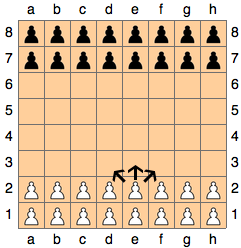
\includegraphics[scale=0.5]{fig1.png}
\caption{Movimento possível da peça e2}
\label{fig:1}
\end{center}
\end{figure}

%Figura 2 (a e b)
\begin{figure}[H]
\begin{center}
\subfloat[Possibilidades para a peça f3]{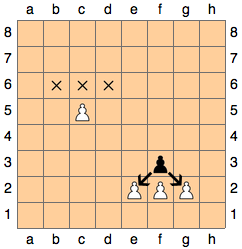
\includegraphics[scale=0.5]{fig2a.png}\label{fig:2a}}\hspace{10px}
\subfloat[Captura de e2]{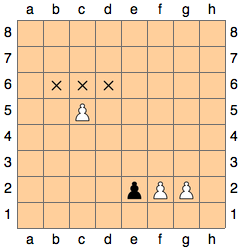
\includegraphics[scale=0.5]{fig2b.png}\label{fig:2b}}
\caption{Processo de captura.}
\label{fig:2}
\end{center}
\end{figure}

\subsection{Vitória}
\begin{enumerate}
\item O primeiro jogador a atingir a base do adversário, vence. No caso anterior, se o jogador 2 (peças pretas) atingisse a linha 1, venceria.
\item Se todas as peças de um jogador forem capturadas, este perde o jogo.
\item Um empate é matemáticamente impossível, e todas as peças têm sempre pelo menos uma jogada na diagonal possível.
\end{enumerate}


%************************************************************************************************
%************************************************************************************************
 
\section{Representação do Estado do Jogo}

A representação do tabuleiro 8x8 é feita em Prolog por uma lista de listas.
Cada item do tabuleiro é representado no formato ``Jogador", em que este pode ser:
\begin{itemize}
\item 1 - jogador de peças brancas (Norte)
\item 2 - jogador de peças pretas (Sul)
\item 0 - casa vazia
\end{itemize}

\begin{code}[H]
	\begin{verbatimtab}
initBoard(
	[
		[ 1, 1, 1, 1, 1, 1, 1, 1 ],
		[ 1, 1, 1, 1, 1, 1, 1, 1 ],
		[ 0, 0, 0, 0, 0, 0, 0, 0 ],
		[ 0, 0, 0, 0, 0, 0, 0, 0 ],
		[ 0, 0, 0, 0, 0, 0, 0, 0 ],
		[ 0, 0, 0, 0, 0, 0, 0, 0 ],
		[ 2, 2, 2, 2, 2, 2, 2, 2 ],
		[ 2, 2, 2, 2, 2, 2, 2, 2 ]
	]).
\end{verbatimtab}
\caption{Representação de tabuleiro inicial.}
\end{code}


\begin{code}[H]
	\begin{verbatimtab}

intermediumBoard(
	[
		[ 1, 1, 1, 1, 1, 1, 1, 1 ],
		[ 1, 1, 0, 1, 1, 1, 0, 1 ],
		[ 0, 0, 1, 0, 0, 0, 0, 0 ],
		[ 0, 0, 0, 0, 0, 1, 0, 0 ],
		[ 0, 0, 0, 0, 0, 2, 0, 0 ],
		[ 0, 0, 0, 2, 0, 0, 0, 2 ],
		[ 2, 2, 2, 0, 2, 0, 0, 2 ],
		[ 2, 2, 2, 2, 2 ,2 ,2, 2 ]
	]).
\end{verbatimtab}
\caption{Representação de tabuleiro intermédio.}
\end{code}


\begin{code}[H]
	\begin{verbatimtab}

finalBoard(
	[
		[ 1, 1, 1, 1, 1, 1, 1, 1 ],
		[ 1, 1, 0, 1, 1, 0, 0, 1 ],
		[ 0, 0, 1, 0, 0, 0, 0, 0 ],
		[ 0, 0, 0, 0, 0, 0, 0, 0 ],
		[ 0, 2, 0, 0, 0, 1, 0, 0 ],
		[ 0, 0, 0, 2, 0, 0, 0, 2 ],
		[ 2, 2, 0, 0, 2, 0, 0, 2 ],
		[ 2, 2, 2, 1, 2, 2, 2, 2 ]
	]).
\end{verbatimtab}
\caption{Representação de tabuleiro final, em que o jogador 1 venceu.}
\end{code}


%************************************************************************************************
%************************************************************************************************
\newpage

\section{Representação de um Movimento}

% Descrever a forma de representação dos diversos tipos de jogadas (movimentos) permitidos no jogo.
% Só é necessário apresentar os cabeçalhos dos predicados que serão utilizados para as diferentes jogadas (que ainda não precisam de estar implementados).

A descrição seguinte será feita tomando o jogador 2 (que avança na direcção Sul-Norte) como referência.

O jogador pode mover uma dada peça sua para uma casa adjacente a:
\begin{enumerate}
\item Norte, se esta estiver vazia.
\item Noroeste ou Nordeste, se esta estiver vazia ou contiver uma peça do oponente, sendo que neste último caso há forçosamente uma captura.
\end{enumerate}
Para efetuar um movimento, chamamos a seguinte função:
\begin{code}[H]
	\begin{verbatimtab}

	movePawn([Ox,Oy], [Dx,Dy]).
\end{verbatimtab}
\caption{Predicado para mover a peça.}
\end{code}
Esta função aceita o X e Y da casa de origem e da casa de destino, e terá de verificar se ambas as casas são adjacentes, bem como validar a jogada, consoante o jogador que estiver na casa de origem.

\begin{code}[H]
	\begin{verbatimtab}

	movePawn([ 7, 5 ], [ 6 , 4 ]).
\end{verbatimtab}
\caption{Exemplificação de um movimento.}
\end{code}
A peça que se encontra em (7, 5), é movida para a casa (6, 4).
\linebreak \linebreak
  Para capturar uma peça do adversário na casa de destino, será usado o seguinte predicado:

\begin{code}[H]
	\begin{verbatimtab}

	capturePawn([Dx, Dy]).
\end{verbatimtab}
\caption{Captura de peça na casa de destino.}
\end{code}



%************************************************************************************************
%************************************************************************************************

\section{Visualização do Tabuleiro}

% Descrever a forma de visualização do tabuleiro em modo de texto e os predicados Prolog construídos para o efeito.
% O código (predicado) desenvolvido, deve receber como parâmetro a representação do tabuleiro (estado do jogo) e permitir visualizar, no ecrã, em modo de texto, o estado do jogo.
% Deve ser incluída no relatório, pelo menos, uma imagem demonstrando a visualização em modo de texto do tabuleiro.

O tabuleiro do jogo, é apresentado no ecrã através do predicado ``printBoard''.
Esta função apresenta as células do tabuleiro representadas pelo número do jogador correspondente, ou em branco, caso a mesma se encontre vazia.
Apresenta também as linhas e colunas à volta do tabuleiro, numeradas do número 1 até ao número da ordem de colunas ou linhas.

% Figura do tabuleiro
\begin{figure}[h!]
\begin{center}
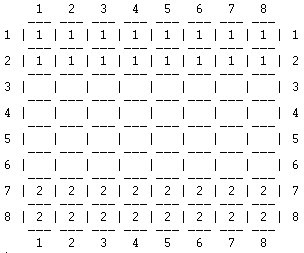
\includegraphics[scale=1]{fig_tab.png}
\caption{Tabuleiro impresso com ``printBoard', mostrando o estado inicial de um jogo'.}
\label{fig:3}
\end{center}
\end{figure}

Na construção do código para esta função, ``printBoard'', foram criados os seguintes predicados:

\begin{code}[H]
	\begin{verbatimtab}

% Imprime a peça do jogador correspondente.
writePlayer(1) :-
	write('1').
writePlayer(2) :-
	write('2').
writePlayer(0) :-
	write(' ').
\end{verbatimtab}
\caption{Predicado ``writePlayer' .}
\end{code}



\begin{code}[H]
	\begin{verbatimtab}

% Critério de paragem.
printRow([]).

% Imprime a borda esquerda da célula, e a respetiva
% peça do jogador (cabeça da lista).
% Por fim chama recursivamente a mesma função com
% a cauda da lista, até encontrar o critério de paragem.
printRow([H|T]) :-
	write('| '),
	writePlayer(H),
	write(' '),
	printRow(T).
\end{verbatimtab}
\caption{Predicado ``printRow'' .}
\end{code}



\begin{code}[H]
	\begin{verbatimtab}

% Imprime a linha de separação horizontal.
printHorizSep   :-
	write('   --- --- --- --- --- --- --- ---').

% Imprime os números das colunas.
printColNumbers :-
	write('    1   2   3   4   5   6   7   8').
\end{verbatimtab}
\caption{Predicado ``printHorizSep'' e ``printColNumbers''.}
\end{code}



\begin{code}[H]
	\begin{verbatimtab}

% Critério de paragem.
printFullRow([], _).

% Imprime o número da linha no ínicio e no fim de cada iteração,
% bem como o separador horizontal. Chama também o predicado que irá
% imprimir todas as células de cada linha, com a respectiva peça.
% Por fim chama recursivamente a mesma função com a cauda da
% lista (contendo as restantes células da linha correspondente),
% e o número actual da linha, até atingir o critério de paragem.
printFullRow([H|T], N) :-
	N1 is N+1,
	printHorizSep,
	nl,
	write(N),
	write(' '),
	printRow(H),
	write('| '),
	write(N),
	nl,
	printFullRow(T, N1).
\end{verbatimtab}
\caption{Predicado ``printFullRow''.}
\end{code}



\begin{code}[H]
	\begin{verbatimtab}

% Regra a ser usada quando é passado um tabuleiro vazio.
printBoard([]).

% Imprime o tabuleiro, chamando o predicado que imprime o número
% das colunas (no início e no fim do tabuleiro),
% e de seguida o predicado que imprime cada linha individual.
% É impresso também o separador horizontal do tabuleiro.
printBoard([H|T]) :-
	printColNumbers,
	nl,
	printFullRow([H|T], 1),
	printHorizSep,
	nl,
	printColNumbers.
\end{verbatimtab}
\caption{Predicado ``printBoard''.}
\end{code}


%************************************************************************************************
%************************************************************************************************
\newpage

\section{Conclusões e Perspectivas de Desenvolvimento}

% Que conclui da análise do jogo e da pesquisa bibliográfica realizada?
% Como vai ser desenvolvido o trabalho?
% Que parte (\%) do trabalho estima que falta fazer?

Dados os conhecimentos adquiridos, podemos concluir que o código dos predicados para efetuar quer um movimento, quer uma captura, deverá ser simples de implementar. 
O trabalho já começou a ser desenvolvido em Prolog, e posteriormente será criado um interface em ambiente gráfico no contexto de LAIG.

Por enquanto, a implementação incidirá apenas no ambiente em modo de texto.

Estimamos que cerca de 15\% do total do projeto esteja concluído, uma vez que os modos de jogo Humano/Computador e Computador/Computador, sendo baseadas na implementação de algoritmos de inteligência artificial, irão necessitar de mais investigação, e por conseguinte mais tempo dispendido.

Olhando otimisticamente para o projeto, achamos que a sua relativa simplicidade nos permitirá desenvolver a lógica de jogo suficientemente depressa para nos podermos concentrar em pequenos detalhes que tornarão o jogo o mais interessante possível.


%************************************************************************************************
%************************************************************************************************

\clearpage

\addcontentsline{toc}{section}{Bibliografia}
\renewcommand\refname{Bibliografia}
\bibliographystyle{plain}
\bibliography{myrefs}

\nocite{breakSite}
\nocite{tut1}
\nocite{tut2}


%************************************************************************************************
%************************************************************************************************
\newpage

\appendix
\section{Código Prolog}

\begin{code}[H]
	\begin{verbatimtab} % verbatimtab para codigo com tabs
initBoard([[ 1, 1, 1, 1, 1, 1, 1, 1 ],
	   [ 1, 1, 1, 1, 1, 1, 1, 1 ],
	   [ 0, 0, 0, 0, 0, 0, 0, 0 ],
	   [ 0, 0, 0, 0, 0, 0, 0, 0 ],
	   [ 0, 0, 0, 0, 0, 0, 0, 0 ],
	   [ 0, 0, 0, 0, 0, 0, 0, 0 ],
	   [ 2, 2, 2, 2, 2, 2, 2, 2 ],
	   [ 2, 2, 2, 2, 2, 2, 2, 2 ]]).
writePlayer(1) :-
	write('1').
writePlayer(2) :-
	write('2').
writePlayer(0) :-
	write(' ').
printRow([]).
printRow([H|T]) :-
	write('| '),
	writePlayer(H),
	write(' '),
	printRow(T).
printHorizSep   :-
	write('   --- --- --- --- --- --- --- ---').
printColNumbers :-
	write('    1   2   3   4   5   6   7   8').
printFullRow([], _).
printFullRow([H|T], N) :-
	N1 is N+1,
	printHorizSep,
	nl,
	write(N),
	write(' '),
	printRow(H),
	write('| '),
	write(N),
	nl,
	printFullRow(T, N1).
printBoard([]).
printBoard([H|T]) :-
	printColNumbers,
	nl,
	printFullRow([H|T], 1),
	printHorizSep,
	nl,
	printColNumbers.
init :-
	initBoard(A),
	printBoard(A).
% Protótipos do predicados da função de movimento e captura de uma peça.
% movePawn([Ox, Oy], [Dx, D2]).
% capturePawn([Dx, Dy]).
\end{verbatimtab}
\caption{Código dos predicados utilizados.}
\end{code}

\end{document}
